\chapter{Introduction}\label{chap:introduction}

The vulnerable bank app simulates a typical online banking environment, complete with features such as user authentication, account management, fund transfers, and transaction history. Despite its realistic functionality, the application is intentionally engineered with several well-known security vulnerabilities, including SQL Injection (SQLi), Cross-Site Scripting (XSS), and Cross-Site Request Forgery (CSRF). 
These vulnerabilities are prevalent in many real-world applications and can have devastating consequences if exploited.
\begin{figure}[H]
	\centering
	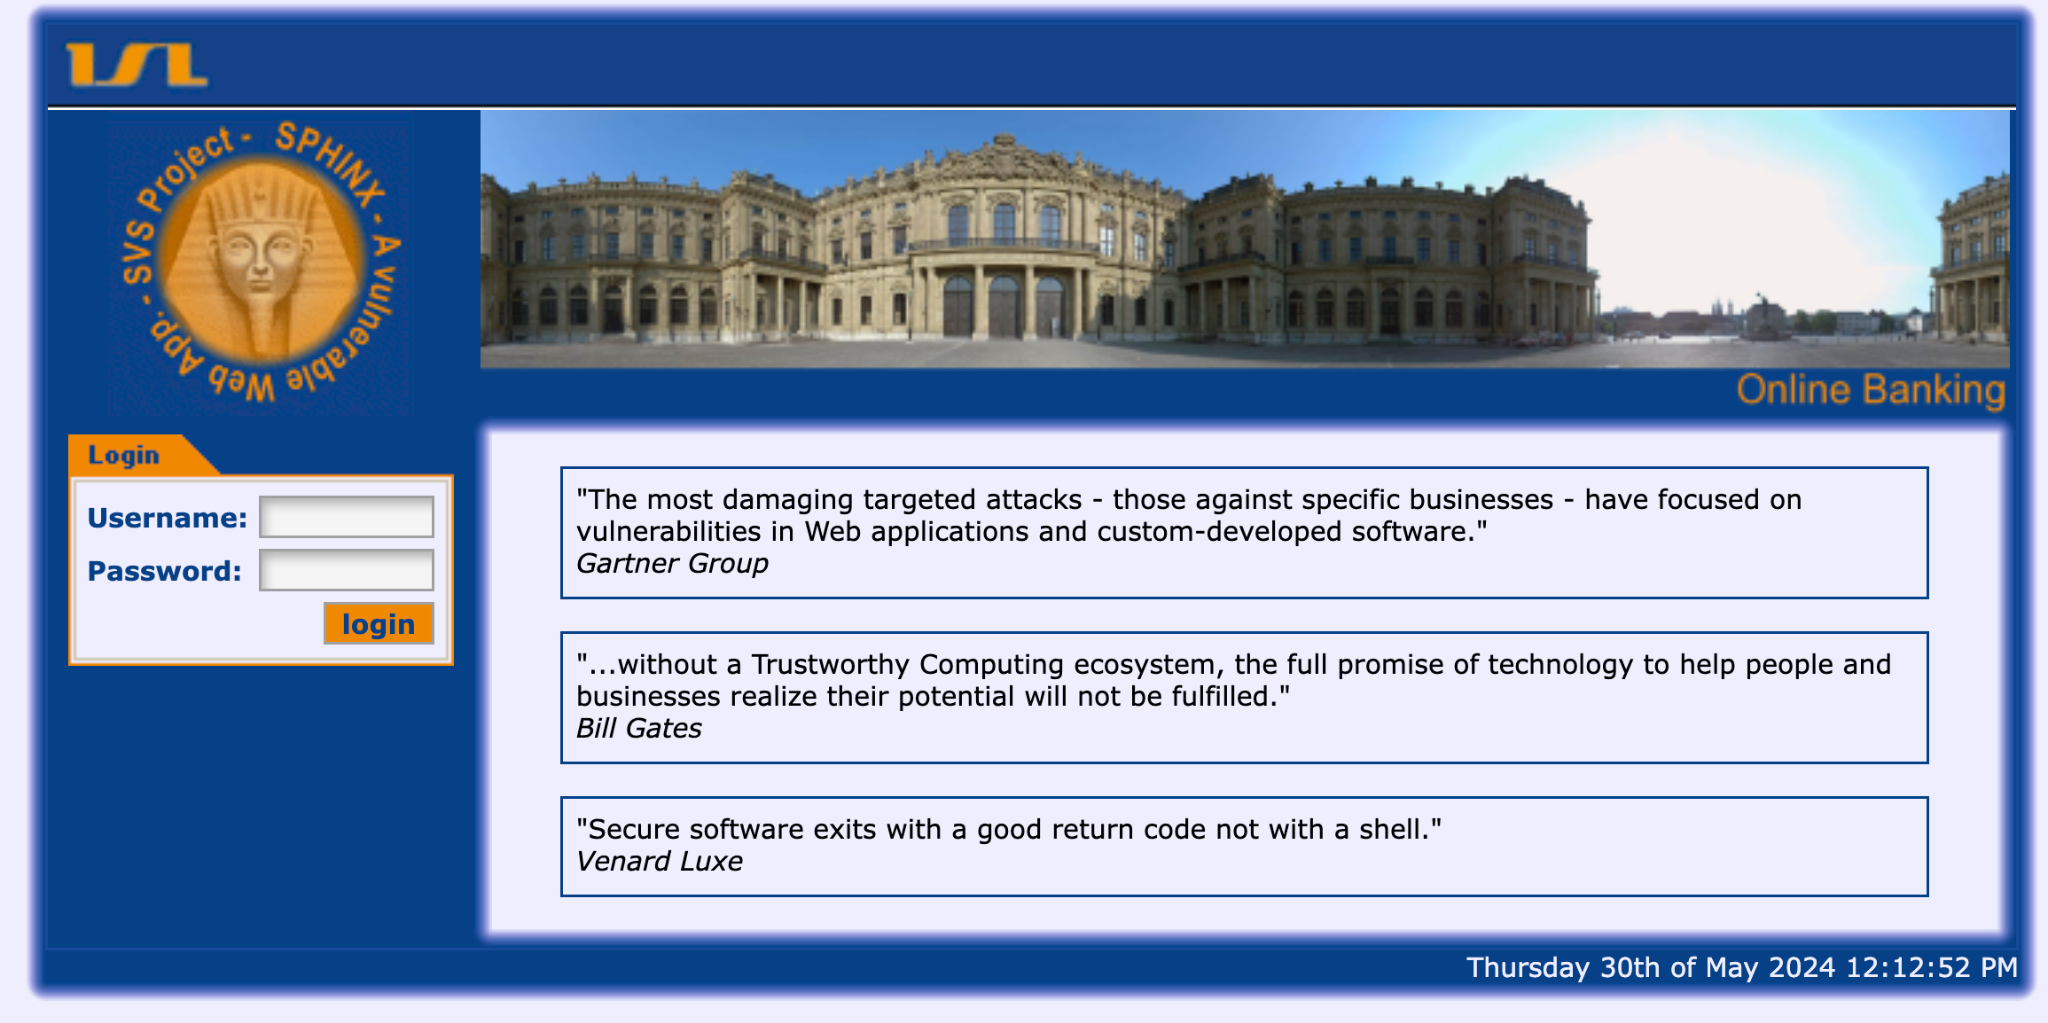
\includegraphics[width=0.5\linewidth]{image11.png}
	\caption{First page Demonstration}
	\label{fig:image1}
\end{figure}
In the provided screenshot we can conclude that this application has two input fields and a login system. The first field is username and the second field is password. 
As an attacker, we need to understand how this application works and figure out the source code behind it. 
Specification of this lab exercise mentions that this app uses PHP with apache2 web server and MySQL database. After following all steps for the installation, we can successfully run this application. 
The web application is served on bank.atiqullah.dev.
